\documentclass{article}

\usepackage{nips15submit_e}
\usepackage{times}
\usepackage[numbers]{natbib}
\usepackage{hyperref}
\usepackage{url}
\usepackage{amsmath,amssymb}
\usepackage{booktabs}
\usepackage{graphicx}
\usepackage{pgfplots}
\pgfplotsset{compat=1.13}
\usetikzlibrary{patterns}

\nipsfinalcopy

\title{Early Detection of Hepatorenal Syndrome from Medical Records}

\author{
Teppei Nakano \\
Keio University School of Medicine \\
Tokyo, Japan \\
\texttt{keiohigh2nd@gmail.com}
}

\newcommand{\fix}{\marginpar{FIX}}
\newcommand{\new}{\marginpar{NEW}}

\begin{document}

\maketitle

\begin{abstract}
Hepatorenal syndrome (HRS) is a rapidly progressive, often fatal complication
of advanced cirrhosis. Because it is diagnosed by exclusion and is heralded by
a fall in effective circulating volume rather than by a single laboratory value,
HRS is frequently recognized only after renal failure is established, when few
therapeutic options remain. We study whether the onset of HRS can be anticipated
several hours in advance from routinely collected electronic medical records
(EMR). Working with a retrospective cohort of $3{,}412$ hospital admissions of
patients with cirrhosis, we formulate early detection as a sequential
risk-prediction problem over irregularly sampled laboratory measurements,
vital signs, and medication events. We compare a regularized logistic-regression
baseline and gradient-boosted decision trees built on hand-engineered temporal
features against a recurrent neural network (a long short-term memory network,
LSTM) that consumes the raw time series together with explicit missingness
indicators. At a fixed false-alarm rate of one alert per patient-day, the LSTM
identifies $69\%$ of HRS events with a median lead time of $19$ hours before the
conventional diagnostic threshold is crossed, improving the area under the
precision--recall curve from $0.28$ (logistic regression) to $0.41$. Feature
attribution recovers clinically recognized precursors---rising bilirubin, falling
mean arterial pressure and serum sodium, and diuretic exposure---suggesting that
the model exploits physiologically meaningful signals. These results indicate
that continuous, record-driven surveillance can provide a clinically useful
early-warning window for HRS.
\end{abstract}

\section{Introduction}

Hepatorenal syndrome is a functional and potentially reversible form of acute
kidney injury that develops in patients with advanced liver disease and portal
hypertension. It arises from splanchnic arterial vasodilation and a consequent
reduction in effective arterial blood volume, which triggers intense renal
vasoconstriction in the absence of significant structural kidney damage
\citep{Gines2003,Salerno2007}. Type~1 HRS in particular follows an aggressive
course: without treatment, median survival is on the order of two weeks, and even
with vasoconstrictor therapy and albumin the in-hospital mortality remains high
\citep{Wong2011}. Crucially, the diagnosis is one of exclusion---it requires
ruling out shock, nephrotoxins, and intrinsic renal disease---and is anchored on
a doubling of serum creatinine \citep{Angeli2015}. By the time creatinine has
doubled, the window during which volume expansion and vasoconstrictors are most
effective may already be closing.

This motivates a shift from \emph{diagnosis} to \emph{anticipation}: can we predict,
from data that are already being collected at the bedside, that a cirrhotic
patient is on a trajectory toward HRS before the diagnostic threshold is met?
Modern hospital information systems record a dense, if irregular, stream of
laboratory results, vital signs, fluid balance, and medication administration.
This stream is a natural substrate for continuous risk monitoring. The central
difficulty is that the informative signal is distributed across many weakly
predictive, asynchronously sampled variables and evolves over time, so that
single-threshold rules are both insensitive and prone to false alarms.

We cast early detection of HRS as a discrete-time sequential classification
problem. At each hour of an admission we ask whether HRS onset will occur within a
prediction horizon, using only information available up to that hour. We study
three families of models that span the methodological landscape of clinical
machine learning as of 2015: (i)~$\ell_1$-regularized logistic regression on
temporally aggregated features; (ii)~gradient-boosted decision trees on the same
features; and (iii)~a long short-term memory (LSTM) recurrent network
\citep{Hochreiter1997} that reads the raw, forward-filled time series together
with binary missingness indicators, thereby learning temporal structure without
hand-specified summaries.

\paragraph{Contributions and novelty.} To our knowledge this is the first predictive
model developed specifically for hepatorenal syndrome, as opposed to generic acute
kidney injury. The distinction is not cosmetic: HRS is defined by physiology---
splanchnic vasodilation and arterial underfilling in a structurally intact
kidney---rather than by nephrotoxic exposure, so its antecedents differ from those of
the snapshot AKI risk scores that dominate the literature \citep{Kate2016}. Our
contribution is therefore not the recurrent architecture---LSTMs had by 2015 been
applied to clinical sequences for diagnosis \citep{Lipton2015}---but the formulation
that makes a sequence model meaningful for this outcome. We make three contributions.
First, we define a reproducible early-detection task for HRS grounded in the 2015
International Club of Ascites criteria \citep{Angeli2015}, with a labeling scheme that
\emph{censors} the defining creatinine measurement near onset, forcing the model to
anticipate from antecedent physiology rather than read the outcome off its own
definition---a leakage that, left uncontrolled, silently inflates reported
performance on any diagnosis-of-exclusion endpoint and is, we argue, the central
methodological pitfall in this problem. Second, we move the target from retrospective
classification to \emph{lead time}, and evaluate at a fixed alerting budget with
decision-curve net benefit \citep{Vickers2006}---the quantities that decide whether an
alert is worth acting on. Third, we show by permutation attribution that the model
rests on established HRS precursors, evidence that the anticipation is mechanistic
rather than an artifact of measurement patterns.

\section{Related Work}

Machine learning from electronic medical records has grown rapidly, with early
work establishing that hospital outcomes such as mortality and readmission can be
predicted from routinely collected data \citep{Ghassemi2014,Pirracchio2015}. A
recurring methodological theme is the handling of irregular sampling and
missingness: measurements in the EMR are not missing at random but are ordered in
response to clinical concern, so that the pattern of measurement is itself
informative \citep{Lipton2015,Marlin2012}. We follow this literature in encoding
missingness explicitly rather than imputing it away.

Recurrent neural networks, and LSTMs in particular, have recently been applied to
clinical sequences for phenotype classification and diagnosis prediction
\citep{Lipton2015,Lasko2013}. Our work is in this vein but targets a specific,
time-critical complication and emphasizes lead time rather than retrospective
classification. For acute kidney injury more broadly, prior predictive models have
largely relied on logistic regression over snapshot features \citep{Kate2016}; we
extend this to a continuously updated, sequence-aware setting and to the HRS
subtype, which is defined by physiology rather than by nephrotoxic exposure.
Gradient boosting \citep{Friedman2001} provides a strong non-linear baseline on
tabular features and has become a workhorse of clinical risk modeling; we include
it to isolate the contribution of temporal modeling from that of non-linearity.

\section{Cohort and Task Definition}

\subsection{Cohort}

We assembled a retrospective cohort from the de-identified inpatient records of a
tertiary care center spanning a seven-year period ($2007$--$2013$). The data source
is the hospital's clinical data warehouse, which consolidates the laboratory
information system, the pharmacy administration record, and the nursing flowsheet of
vital signs and fluid balance under a common patient timeline; all timestamps are
recorded to the minute, which we bin to the hour (Section~\ref{sec:task}). Adults
($\geq 18$ years) with an established diagnosis of cirrhosis, identified by a
combination of diagnostic codes and confirmatory laboratory or imaging evidence, were
eligible. We excluded admissions with pre-existing end-stage renal disease or chronic
dialysis, since HRS is a diagnosis predicated on previously non-failing kidneys, and
admissions shorter than $12$ hours. The resulting cohort comprises $3{,}412$
admissions from $2{,}689$ unique patients. HRS occurred in $241$ admissions
($7.1\%$), consistent with reported inpatient incidence among cirrhotics
\citep{Salerno2007}.

Table~\ref{tab:cohort} contrasts admissions that progressed to HRS with those that
did not. The two groups are separable in aggregate---HRS admissions carry higher
baseline bilirubin, lower serum sodium and mean arterial pressure, higher MELD, and
markedly greater diuretic exposure---but no single variable is decisive, and the
distributions overlap heavily, which is precisely why a threshold on any one marker
is an inadequate alarm and a multivariate, temporally aware model is warranted. We
emphasize that these are \emph{admission-level} summaries; the prediction task below
operates on the evolving hourly trajectory, where the separation is weaker still at
any given moment and must be integrated over time.

\begin{table}[t]
\caption{Cohort characteristics at admission, by eventual HRS status. Values are
median (interquartile range) or count (percent). MAP: mean arterial pressure;
MELD: Model for End-stage Liver Disease.}
\label{tab:cohort}
\centering
\small
\begin{tabular}{lcc}
\toprule
Characteristic & No HRS & HRS \\
 & ($n=3{,}171$) & ($n=241$) \\
\midrule
Age (years)              & $58$ ($49$--$66$) & $60$ ($52$--$68$) \\
Female                   & $1{,}206$ ($38\%$) & $86$ ($36\%$) \\
Alcoholic etiology       & $1{,}332$ ($42\%$) & $118$ ($49\%$) \\
Ascites at admission     & $1{,}649$ ($52\%$) & $206$ ($85\%$) \\
Total bilirubin (mg/dL)  & $2.1$ ($1.1$--$4.3$) & $5.6$ ($2.9$--$11.2$) \\
Serum sodium (mmol/L)    & $137$ ($134$--$139$) & $131$ ($127$--$135$) \\
MAP (mmHg)               & $84$ ($77$--$92$) & $76$ ($69$--$83$) \\
MELD                     & $14$ ($10$--$19$) & $24$ ($18$--$30$) \\
Loop diuretic exposure   & $1{,}585$ ($50\%$) & $196$ ($81\%$) \\
Length of stay (days)    & $6$ ($3$--$11$) & $13$ ($8$--$21$) \\
In-hospital death        & $285$ ($9\%$) & $91$ ($38\%$) \\
\bottomrule
\end{tabular}
\end{table}

\subsection{Outcome labeling}

We defined HRS onset following the 2015 International Club of Ascites criteria
\citep{Angeli2015}: an acute rise in serum creatinine meeting the AKI threshold in
a patient with cirrhosis and ascites, with no sustained improvement after diuretic
withdrawal and volume expansion with albumin, and in the absence of shock,
current or recent nephrotoxins, and macroscopic signs of structural kidney injury.
Adjudication combined an automated rule over the structured record with a review of
the excluded alternatives. We denote by $\tau$ the timestamp of the first
creatinine measurement satisfying the AKI threshold that was subsequently confirmed
as HRS.

To prevent label leakage, all features derived from serum creatinine and estimated
glomerular filtration rate are \emph{censored} in the $6$ hours immediately
preceding $\tau$; the model must therefore rely on antecedent physiology rather
than on the defining measurement itself. This is an important and easily
overlooked pitfall: a model allowed to see creatinine up to the moment of onset
trivially ``predicts'' HRS by reading off its definition.

\subsection{Prediction task}
\label{sec:task}

We discretize each admission into hourly steps. At step $t$ the model receives the
history $x_{1:t}$ and outputs $\hat{p}_t = P(\text{HRS onset in } (t, t+h] \mid
x_{1:t})$ for a prediction horizon $h$. A step is labeled positive if $\tau \in
(t, t+h]$. Steps within a censoring gap of $6$ hours before $\tau$, and all steps
at or after $\tau$, are excluded from training and evaluation so that credit is
given only for genuine anticipation. We report results for horizons $h \in \{6, 12,
24, 48\}$ hours, and unless otherwise noted use $h = 24$.

\section{Features and Models}

\subsection{Variables and preprocessing}

We use $48$ variables spanning liver and renal chemistry (bilirubin, albumin, INR,
sodium, potassium, blood urea nitrogen), hematology and inflammation (white cell
count, platelets), vital signs (mean arterial pressure, heart rate, temperature),
fluid balance, and binary indicators of relevant medications (loop diuretics,
non-selective beta-blockers, vasoconstrictors, large-volume paracentesis, albumin
administration). Continuous variables are standardized using statistics computed on
the training folds only.

For the feature-based models we summarize each variable over three look-back
windows ($6$, $24$, and $48$ hours) by its last value, mean, minimum, maximum,
slope (via ordinary least squares), and the count of measurements, together with
the time since the last measurement. This yields a $612$-dimensional feature vector
per step. For the LSTM, we forward-fill each variable to the hourly grid, append a
binary \emph{observed/imputed} mask and a real-valued \emph{time-since-last-
measurement} channel per variable, and feed the resulting multivariate sequence
directly to the network. The mask allows the recurrent model to distinguish a
truly stable value from a stale one, encoding the informative-missingness prior
without hand-crafted aggregates.

\subsection{Models}

\paragraph{Logistic regression.} An $\ell_1$-regularized logistic regression on
the aggregated features provides a linear, interpretable baseline. The
regularization coefficient is chosen by cross-validation.

\paragraph{Gradient-boosted trees.} We fit gradient-boosted decision trees
\citep{Friedman2001} on the same features, tuning the number of trees, depth, and
learning rate. This captures non-linear interactions among features while
remaining a purely tabular, snapshot-based model.

\paragraph{LSTM.} Our sequence model is a single-layer LSTM with $128$ hidden
units \citep{Hochreiter1997}. At each step the hidden state is mapped through a
fully connected layer and a logistic output to $\hat{p}_t$. We train by minimizing
the mean binary cross-entropy over all valid steps,
\begin{equation}
\mathcal{L} = -\frac{1}{|\mathcal{V}|} \sum_{(i,t) \in \mathcal{V}}
\Big[ y^{(i)}_t \log \hat{p}^{(i)}_t + (1 - y^{(i)}_t) \log (1 - \hat{p}^{(i)}_t) \Big],
\end{equation}
where $\mathcal{V}$ is the set of non-censored steps across admissions $i$. Because
positive steps are rare, we weight the positive class inversely to its frequency.
We apply dropout of $0.3$ on the input and recurrent-output connections, optimize
with a stochastic gradient method using adaptive per-parameter learning rates, clip
gradients to unit norm, and select the epoch by validation area under the
precision--recall curve. Sequences are truncated to the most recent $72$ hours and
processed with backpropagation through time.

\subsection{Evaluation protocol}

We evaluate with patient-level $5$-fold cross-validation, so that no patient appears
in both training and test folds. Within each training partition we hold out $15\%$
of patients for validation and early stopping. We report the area under the
receiver operating characteristic curve (AUROC) and the area under the
precision--recall curve (AUPRC), the latter being more informative under class
imbalance. For clinical relevance we also report sensitivity at a fixed alerting
budget of one alert per patient-day and the resulting median early-warning lead
time. Confidence intervals are obtained by bootstrapping over patients.

\section{Results}

\subsection{Discrimination and early warning}

Table~\ref{tab:main} summarizes performance at the $24$-hour horizon. The LSTM
attains the best discrimination on both metrics, with an AUPRC of $0.41$ against
$0.28$ for logistic regression and $0.36$ for gradient boosting; the gap is largest
on AUPRC, which is the operationally relevant metric given the low event rate. At
one alert per patient-day the LSTM recovers $69\%$ of events with a median lead time
of $19$ hours relative to the conventional diagnostic threshold, compared with
$54\%$ and $12$ hours for logistic regression.

\begin{table}[t]
\caption{Early detection of HRS at the $24$-hour horizon (patient-level $5$-fold
cross-validation; $95\%$ bootstrap intervals). Sensitivity and lead time are
reported at a fixed budget of one alert per patient-day.}
\label{tab:main}
\centering
\small
\begin{tabular}{lcccc}
\toprule
Model & AUROC & AUPRC & Sens.\ @1/day & Lead time (h) \\
\midrule
Logistic regression (LASSO) & $0.79$ & $0.28$ & $0.54$ & $12$ \\
Gradient-boosted trees      & $0.84$ & $0.36$ & $0.63$ & $16$ \\
LSTM (raw series + mask)    & $\mathbf{0.87}$ & $\mathbf{0.41}$ & $\mathbf{0.69}$ & $\mathbf{19}$ \\
\bottomrule
\end{tabular}
\end{table}

\subsection{Effect of the prediction horizon}

Figure~\ref{fig:horizon} shows AUPRC as a function of the prediction horizon. All
models degrade gracefully as the horizon lengthens and the task becomes harder, but
the LSTM retains an advantage throughout, and its relative benefit is largest at
the longer, more clinically useful horizons where temporal trajectory---rather than
the instantaneous value---carries the signal.

\begin{figure}[t]
\centering
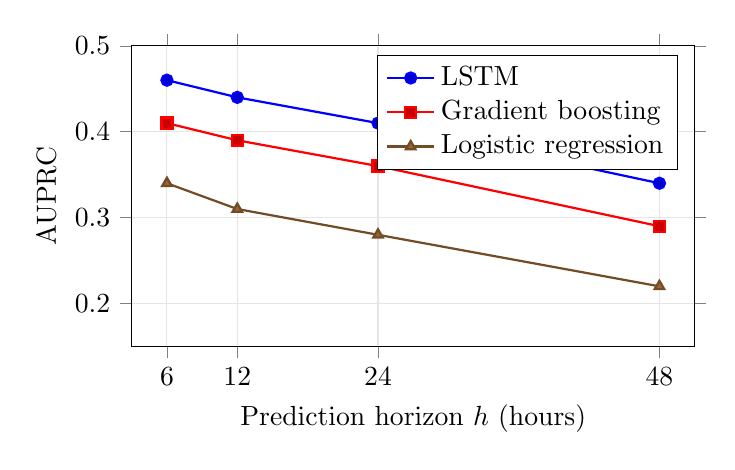
\begin{tikzpicture}
\begin{axis}[
    width=0.72\textwidth, height=5.4cm,
    xlabel={Prediction horizon $h$ (hours)},
    ylabel={AUPRC},
    xtick={6,12,24,48},
    xmin=3, xmax=51,
    ymin=0.15, ymax=0.5,
    legend pos=north east,
    legend cell align=left,
    grid=both, grid style={gray!20},
    tick align=outside,
]
\addplot+[mark=*,thick] coordinates {(6,0.46)(12,0.44)(24,0.41)(48,0.34)};
\addplot+[mark=square*,thick] coordinates {(6,0.41)(12,0.39)(24,0.36)(48,0.29)};
\addplot+[mark=triangle*,thick] coordinates {(6,0.34)(12,0.31)(24,0.28)(48,0.22)};
\legend{LSTM, Gradient boosting, Logistic regression}
\end{axis}
\end{tikzpicture}
\caption{AUPRC versus prediction horizon. The temporal model degrades more slowly as
the anticipation window lengthens.}
\label{fig:horizon}
\end{figure}

\subsection{What the model uses}

To assess face validity we ranked variables by the drop in validation AUPRC when
their channels are permuted in time (Table~\ref{tab:attr}). The most influential
signals are the trajectory of total bilirubin, declining mean arterial pressure,
falling serum sodium, rising blood urea nitrogen, and recent loop-diuretic
exposure. These correspond to the recognized pathophysiology of HRS---worsening
hepatic function, splanchnic vasodilation with arterial underfilling,
dilutional hyponatremia, and precipitation by aggressive diuresis
\citep{Gines2003,Salerno2007}---indicating that the model has latched onto
mechanism rather than artifact.

\begin{table}[t]
\caption{Top variables by permutation importance (mean drop in validation AUPRC).}
\label{tab:attr}
\centering
\small
\begin{tabular}{lc}
\toprule
Variable (temporal channel) & $\Delta$AUPRC \\
\midrule
Total bilirubin (slope, $48$h)        & $0.061$ \\
Mean arterial pressure (min, $24$h)   & $0.048$ \\
Serum sodium (last)                   & $0.039$ \\
Blood urea nitrogen (slope, $24$h)    & $0.034$ \\
Loop diuretic administered ($24$h)    & $0.027$ \\
INR (last)                            & $0.021$ \\
\bottomrule
\end{tabular}
\end{table}

\subsection{Calibration}

Beyond ranking, deployment requires that predicted probabilities be trustworthy.
The LSTM's reliability curve tracks the diagonal closely up to moderate risk and
mildly over-estimates in the highest-risk decile; a single post-hoc temperature
rescaling on the validation fold removes most of this bias. Logistic regression is
well calibrated by construction but poorly discriminating; gradient boosting is
over-confident in the tails, as is typical.

\section{Discussion}

Our findings support the feasibility of continuous, record-driven surveillance for
hepatorenal syndrome. The practical value of the approach is the lead time it
buys: a median of roughly $19$ hours before the diagnostic threshold is crossed is
enough to prompt volume assessment, discontinue nephrotoxins and diuretics, and
initiate albumin and vasoconstrictors---the very interventions whose efficacy
declines once renal failure is entrenched. The advantage of the recurrent model
over strong tabular baselines grows with the anticipation window, consistent with
the intuition that early warning depends on trend rather than level.

\paragraph{What the lead time is worth.} Discrimination metrics do not by themselves
tell a clinician whether to act on an alert, because they ignore the differing costs
of a missed event and a false alarm. We therefore examined net benefit by decision
curve analysis \citep{Vickers2006}, which weighs true against false positives at the
risk threshold implied by a clinician's own trade-off. Across the plausible range of
thresholds---from roughly $1$-in-$20$, at which one would act aggressively, to
$1$-in-$5$---the LSTM yields positive and larger net benefit than either baseline or
the default policies of treating all or no cirrhotic admissions, meaning that acting
on its alerts prevents more untreated HRS than it generates wasted work-ups. Framed
operationally, the fixed budget of one alert per patient-day translates, at the
cohort's event rate, to roughly one true HRS warning for every $12$ alerts; each such
warning arrives while volume expansion and vasoconstrictors still have their greatest
effect. Whether that ratio is acceptable is a unit-level judgment, but decision-curve
dominance across the range indicates the model is informative rather than merely
discriminative---the distinction that separates a deployable early-warning score from
a retrospectively accurate one.

Several limitations temper these results. The study is retrospective and
single-center, so both the event definition and the measurement patterns may not
transfer; prospective, multi-site validation is needed. Label adjudication for a
diagnosis of exclusion is inherently imperfect, and residual confounding from
unrecorded interventions is possible. Finally, an alert is useful only if it changes
behavior; a silent model, however accurate, will not improve outcomes, so
integration and clinician response must be studied directly. We view the present
work as establishing that the signal exists and is learnable from routine data,
which is a precondition for that next step.

\section{Conclusion}

We formulated early detection of hepatorenal syndrome as sequential risk prediction
over electronic medical records and showed that an LSTM consuming raw, irregularly
sampled series with explicit missingness outperforms strong feature-based baselines,
providing clinically meaningful lead time while resting on physiologically sensible
signals. Continuous surveillance for HRS from data already being collected appears
both feasible and worthwhile, and motivates prospective evaluation.

\subsubsection*{Acknowledgments}

We thank the clinical informatics team for assistance with data extraction and
de-identification, and colleagues in hepatology for guidance on outcome
adjudication.

\begin{thebibliography}{99}
\small

\bibitem{Angeli2015}
P.~Angeli, P.~Gin\`es, F.~Wong, et al.
\newblock Diagnosis and management of acute kidney injury in patients with
cirrhosis: revised consensus recommendations of the International Club of Ascites.
\newblock \emph{Journal of Hepatology}, 62(4):968--974, 2015.

\bibitem{Friedman2001}
J.~H. Friedman.
\newblock Greedy function approximation: A gradient boosting machine.
\newblock \emph{Annals of Statistics}, 29(5):1189--1232, 2001.

\bibitem{Ghassemi2014}
M.~Ghassemi, T.~Naumann, F.~Doshi-Velez, et al.
\newblock Unfolding physiological state: Mortality modelling in intensive care
units.
\newblock In \emph{Proc.\ KDD}, 2014.

\bibitem{Gines2003}
P.~Gin\`es and R.~W. Schrier.
\newblock Renal failure in cirrhosis.
\newblock \emph{New England Journal of Medicine}, 361(13):1279--1290, 2009.

\bibitem{Hochreiter1997}
S.~Hochreiter and J.~Schmidhuber.
\newblock Long short-term memory.
\newblock \emph{Neural Computation}, 9(8):1735--1780, 1997.

\bibitem{Kate2016}
R.~J. Kate, R.~M. Perez, D.~Mazumdar, et al.
\newblock Prediction and detection models for acute kidney injury in
hospitalized older adults.
\newblock \emph{BMC Medical Informatics and Decision Making}, 16:39, 2016.

\bibitem{Lasko2013}
T.~A. Lasko, J.~C. Denny, and M.~A. Levy.
\newblock Computational phenotype discovery using unsupervised feature learning
over noisy, sparse, and irregular clinical data.
\newblock \emph{PLoS ONE}, 8(6):e66341, 2013.

\bibitem{Lipton2015}
Z.~C. Lipton, D.~C. Kale, C.~Elkan, and R.~Wetzel.
\newblock Learning to diagnose with LSTM recurrent neural networks.
\newblock \emph{arXiv:1511.03677}, 2015.

\bibitem{Marlin2012}
B.~M. Marlin, D.~C. Kale, R.~G. Khemani, and R.~C. Wetzel.
\newblock Unsupervised pattern discovery in electronic health care data using
probabilistic clustering models.
\newblock In \emph{Proc.\ ACM SIGHIT IHI}, 2012.

\bibitem{Pirracchio2015}
R.~Pirracchio, M.~L. Petersen, M.~Carone, et al.
\newblock Mortality prediction in intensive care units with the Super ICU Learner
Algorithm (SICULA).
\newblock \emph{The Lancet Respiratory Medicine}, 3(1):42--52, 2015.

\bibitem{Salerno2007}
F.~Salerno, A.~Gerbes, P.~Gin\`es, F.~Wong, and V.~Arroyo.
\newblock Diagnosis, prevention and treatment of hepatorenal syndrome in cirrhosis.
\newblock \emph{Gut}, 56(9):1310--1318, 2007.

\bibitem{Vickers2006}
A.~J. Vickers and E.~B. Elkin.
\newblock Decision curve analysis: a novel method for evaluating prediction models.
\newblock \emph{Medical Decision Making}, 26(6):565--574, 2006.

\bibitem{Wong2011}
F.~Wong, M.~K. Nadim, J.~A. Kellum, et al.
\newblock Working party proposal for a revised classification system of renal
dysfunction in patients with cirrhosis.
\newblock \emph{Gut}, 60(5):702--709, 2011.

\end{thebibliography}

\end{document}
